\section{Problem (8)}
	A block of mass $m_{1} = 0.45 \ sl$ on a frictionless plane inclined at angle $\theta = 34^{o}$ is connected by a cord over a massless, frictionless pulley to a second block of mass $m_{2} = 0.15 \ sl$ hanging vertically.

	\begin{figure}[H]
		\begin{center}
			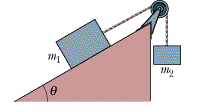
\includegraphics[scale=1]{hw5_problem8}
			\caption{Illustration of Problem 8}
			\label{fig:hw5_problem8}
		\end{center}
	\end{figure}

	\subsection{Question (a)}

		What is the acceleration of the hanging block (choose the positive direction up)?

		\textbf{R:} \newline

		\begin{figure}[H]
			\begin{center}
				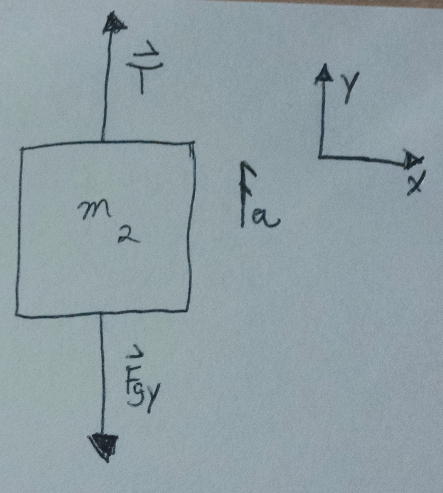
\includegraphics[scale=0.4]{hw5_problem8_fbd}
				\caption{Free-Body Diagram (Problem 8 - Block 1)}
				\label{fig:hw5_problem8_fbd}
			\end{center}
		\end{figure}

		For this problem, we can assume:
		\begin{itemize}
			\item{The tensions in both blocks are equals}
			\item{The aceleration in both blocks have the same magnitude}
		\end{itemize}

		Newton's $2^{nd}$ Law on Block $1$:
		\begin{align}
			\sum F_{x} = \ &m_{1}a_{x}& \notag \\
			T - F_{g_{x}} = \ &(0.45 \ sl)a& \notag \\
			T = \ &(0.45 \ sl)a + F_{g} \sin 34^{o}& \notag \\
			T = \ &(0.45 \ sl)a + (0.45 \ sl)\left(32.2 \ ft/s^{2}\right)(0.559)& \notag \\
			T = \ &(0.45 \ sl)a + 8.1 \ lb& \notag
		\end{align}

		\begin{figure}[H]
			\begin{center}
				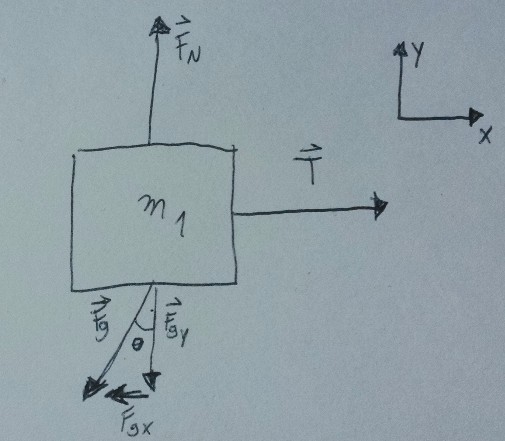
\includegraphics[scale=0.4]{hw5_problem8_2_fbd}
				\caption{Free-Body Diagram (Problem 8 - Block 2)}
				\label{fig:hw5_problem8_2_fbd}
			\end{center}
		\end{figure}

		Newton's $2^{nd}$ Law on Block $2$:
		\begin{align}
			\sum F_{y} = \ &m_{2}a_{y}& \notag \\
			T - F_{g_{y}} = \ &(0.15 \ sl)a& \notag \\
			T = \ &(0.15 \ sl)a + (0.15 \ sl)\left(32.2 \ ft/s^{2}\right)& \notag \\
			T = \ &(0.15 \ sl)a + 14.49 \ lb& \notag
		\end{align}

		\begin{align}
			(0.15 \ sl)a + (14.49 \ lb) = \ &(0.45 \ sl)a + (8.1 \ lb)& \notag \\
			(0.15 \ sl)a - (0.45 \ sl)a = \ &(8.1 \ lb) - (14.49 \ lb)& \notag \\
			-(0.3 \ sl)a = \ &-6.39 \ lb& \notag \\
			a = \ &\frac{-6.39 \ lb}{-0.3 \ sl} = 21.3 \ ft/s^{2}&
		\end{align}

	\subsection{Question (b)}

		What is the tension in the cord?

		\textbf{R:} \newline

		\begin{align}
			T = \ &(0.15 \ sl)\left(21.3 \ ft/s^{2}\right) + 14.49 \ lb& \notag \\
			= \ &(3.19 \ lb) + (14.49 \ lb)& \notag \\
			= \ &17.68 \ lb&
		\end{align}
